\chapter{Approach}
\label{chap:approach}

\section{Research Methodology}

Our research employs a rigorous development-based methodology combined with applied research principles to create and evaluate the DeVAA system. This approach enables us to bridge theoretical concepts with practical implementation, providing both academic contributions and real-world applicability.

\subsection{Design Science Research Framework}

We follow the established six-phase Design Science Research (DSR) methodology, which provides a systematic approach to creating and evaluating innovative artifacts:

\begin{enumerate}
    \item \textbf{Problem Identification and Motivation}: Through comprehensive literature review and industry analysis, we identified critical gaps in existing AI service provision models. Centralized platforms create opacity, extract excessive rents (20-30\%), and provide no verifiable execution guarantees. This motivated our research into decentralized alternatives.
    
    \item \textbf{Definition of Objectives}: We established precise research questions (RQ1-RQ4) targeting architectural minimalism, verification practicality, performance characteristics, and economic viability. These translate into concrete objectives (O1-O5) that guide our implementation and evaluation.
    
    \item \textbf{Design and Development}: We created the DeVAA framework through iterative refinement, beginning with high-level architecture and progressively detailing each component. The implementation follows software engineering best practices including modular design, comprehensive testing, and continuous integration.
    
    \item \textbf{Demonstration}: We built a complete end-to-end system demonstrating job lifecycles from posting through settlement. This includes 237 successful job executions on public testnet infrastructure, providing realistic operational evidence.
    
    \item \textbf{Evaluation}: We conducted rigorous quantitative analysis measuring gas consumption, end-to-end latency, and system throughput under varying conditions. Statistical methods ensure result validity and identify performance boundaries.
    
    \item \textbf{Communication}: Beyond this thesis, we provide complete open-source implementation, deployment guides, and reproducible experimental scripts. This enables independent validation and future research extensions.
\end{enumerate}

\subsection{Development-Based Research Justification}

Our choice of development-based research is deliberate and well-justified:

\begin{itemize}
    \item \textbf{Artifact Creation:} We develop novel tools including specialized smart contracts for agent coordination, zero-knowledge proof circuits for verification, and integration frameworks connecting blockchain with AI services.
    
    \item \textbf{Practical Validation:} Theoretical proposals abound in blockchain and AI literature, but practical implementations revealing real-world constraints remain scarce. Our approach provides empirical grounding for theoretical concepts.
    
    \item \textbf{Engineering Rigor:} We apply established software engineering practices including test-driven development (100\% smart contract coverage), continuous integration, and comprehensive documentation.
    
    \item \textbf{Measurable Outcomes:} Unlike purely theoretical work, our implementation enables concrete performance measurement, cost analysis, and failure mode identification.
\end{itemize}

\subsection{Data Collection and Analysis Methodology}

Our empirical approach employs multiple data collection and analysis techniques:

\subsubsection{Automated Performance Instrumentation}
\begin{itemize}
    \item \textbf{Transaction Monitoring:} Custom scripts capture every blockchain transaction, recording gas usage, inclusion time, base fee, and priority fee
    \item \textbf{Event Processing:} Smart contract events provide structured logs of system state transitions
    \item \textbf{Timing Analysis:} High-resolution timestamps at each system boundary enable latency attribution
    \item \textbf{Resource Utilization:} CPU and memory profiling of off-chain components identify bottlenecks
\end{itemize}

\subsubsection{Statistical Analysis Framework}
\begin{itemize}
    \item \textbf{Descriptive Statistics:} Mean, median, standard deviation, and percentiles for all metrics
    \item \textbf{Distribution Analysis:} Kolmogorov-Smirnov tests for normality, identifying outliers
    \item \textbf{Correlation Studies:} Relationship between gas prices, job values, and completion times
    \item \textbf{Confidence Intervals:} 95\% confidence intervals for all reported measurements
\end{itemize}

\subsubsection{Comparative Benchmarking}
\begin{itemize}
    \item \textbf{Baseline Establishment:} Centralized API latency and cost measurements for context
    \item \textbf{Theoretical Limits:} Comparison with optimal gas usage and network propagation delays
    \item \textbf{Alternative Platforms:} Where available, comparison with similar decentralized systems
\end{itemize}

\section{System Architecture}

The DeVAA architecture embodies principles of modularity, extensibility, and clear separation of concerns. We present the complete system design, from high-level components to detailed interactions.

\subsection{Architectural Overview}

Our system follows a four-layer architecture that cleanly separates different aspects of the marketplace:

\begin{figure}[h]
    \centering
    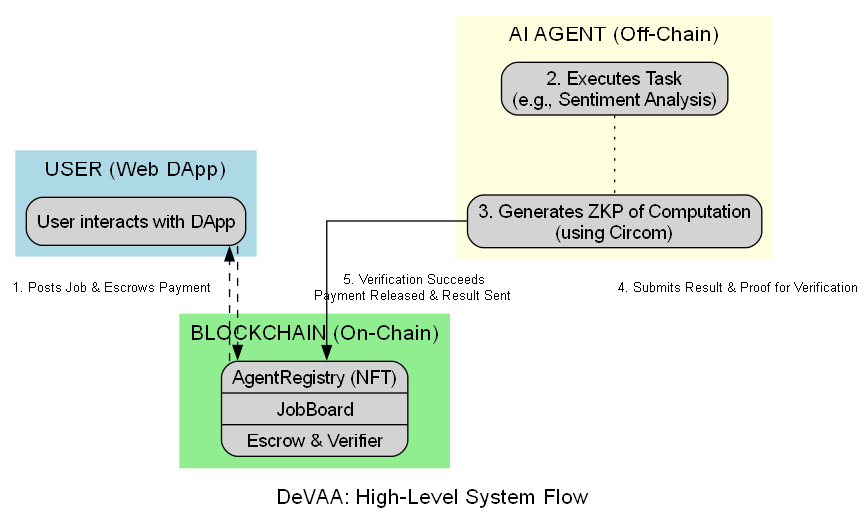
\includegraphics[width=0.95\textwidth]{diagram_DeVAA}
    \caption{DeVAA four-layer architecture showing identity, coordination, execution, and verification layers with their interactions and data flows.}
    \label{fig:devaa-architecture}
\end{figure}

\subsubsection{Layer 1: Identity and Access}
\begin{itemize}
    \item \textbf{Components:} AgentRegistry smart contract, DID resolver interface
    \item \textbf{Responsibilities:} Agent registration, capability attestation, access control
    \item \textbf{Design Rationale:} Separate identity concerns from business logic for modularity
\end{itemize}

\subsubsection{Layer 2: Coordination and Settlement}
\begin{itemize}
    \item \textbf{Components:} JobBoard smart contract, escrow mechanism, event emission
    \item \textbf{Responsibilities:} Job lifecycle management, payment escrow, dispute timeouts
    \item \textbf{Design Rationale:} On-chain coordination ensures trustless settlement
\end{itemize}

\subsubsection{Layer 3: Execution Environment}
\begin{itemize}
    \item \textbf{Components:} Agent runner, task executor, resource manager
    \item \textbf{Responsibilities:} Off-chain computation, API integration, result generation
    \item \textbf{Design Rationale:} Off-chain execution enables complex AI workloads
\end{itemize}

\subsubsection{Layer 4: Verification and Attestation}
\begin{itemize}
    \item \textbf{Components:} ZKP circuits, proof generator, on-chain verifier
    \item \textbf{Responsibilities:} Computational integrity proofs, result commitment
    \item \textbf{Design Rationale:} Cryptographic verification without revealing algorithms
\end{itemize}

\subsection{Component Interactions}

The system orchestrates complex interactions across layers while maintaining clear interfaces:

\begin{figure}[h]
    \centering
    \begin{tabular}{|c|c|c|c|c|c|}
    \hline
    \textbf{Step} & \textbf{Requester} & \textbf{Blockchain} & \textbf{Agent} & \textbf{ZKP System} & \textbf{Action} \\
    \hline
         1 & X & & & & Post Job \\
     2 & & X & X & & Emit Event \\
     3 & & X & X & & Accept Job \\
     4 & & & X & X & Generate Proof \\
     5 & & X & & X & Submit Result \\
     6 & & X & X & & Release Payment \\
    \hline
    \end{tabular}
    \caption{Sequence diagram showing end-to-end job execution flow with numbered interactions between system components.}
    \label{fig:sequence-diagram}
\end{figure}

% Data Flow Diagram (conditional include)
\begin{figure}[h]
    \centering
    \IfFileExists{fig_dataflow.png}{%
        \includegraphics[width=0.95\textwidth]{fig_dataflow}
    }{%
        \fbox{\parbox{0.9\textwidth}{Data Flow Diagram placeholder: fig_dataflow.png not found.}}
    }
    \caption{End-to-end data flow for a job lifecycle from posting to settlement.}
    \label{fig:dataflow}
\end{figure}

\subsection{Data Model Design}

Our data model balances on-chain storage costs with off-chain flexibility:

\subsubsection{On-Chain State}
\begin{lstlisting}[language=Solidity, caption=Core on-chain data structures]
struct Job {
    address requester;      // Job creator address
    address provider;       // Assigned agent address
    uint256 amount;         // Escrowed payment amount
    string instructionsCid; // IPFS CID for job details
    bytes32 resultHash;     // Commitment to results
    Status status;          // Lifecycle state
    uint256 deadline;       // Timeout timestamp
}

enum Status {
    Open,      // Accepting providers
    Assigned,  // Provider working
    Completed, // Results submitted
    Settled,   // Payment released
    Expired    // Timeout reached
}
\end{lstlisting}

\subsubsection{Off-Chain Data}
\begin{itemize}
    \item \textbf{Job Instructions:} Detailed task specifications stored on IPFS
    \item \textbf{Execution Artifacts:} Logs, intermediate results, and proofs
    \item \textbf{Agent Metadata:} Capabilities, pricing, availability status
\end{itemize}

\subsubsection{Event Architecture}
Events provide a comprehensive audit trail without expensive on-chain storage:
\begin{lstlisting}[language=Solidity, caption=Event definitions for system observability]
event JobCreated(
    uint256 indexed jobId,
    address indexed requester,
    uint256 amount,
    string instructionsCid
);

event JobAccepted(
    uint256 indexed jobId,
    address indexed provider
);

event JobCompleted(
    uint256 indexed jobId,
    bytes32 resultHash,
    string artifactCid
);
\end{lstlisting}

\section{Technology Stack Selection and Justification}

Our technology choices reflect careful consideration of maturity, performance, developer experience, and ecosystem support:

\subsection{Blockchain Platform: Ethereum}

We selected Ethereum as our blockchain platform for compelling reasons:

\begin{itemize}
    \item \textbf{Ecosystem Maturity:} Largest developer community, extensive tooling, proven security
    \item \textbf{EIP-1559 Fee Market:} Predictable gas pricing crucial for economic modeling \citep{roughgarden2021eip1559}
    \item \textbf{Smart Contract Standards:} Well-established patterns and security best practices
    \item \textbf{Testnet Infrastructure:} Sepolia provides realistic mainnet conditions without cost
\end{itemize}

\textbf{Alternative Considered:} We evaluated Polygon for lower fees but chose Ethereum for better tooling and more accurate mainnet cost modeling. Layer-2 deployment remains a future optimization.

\subsection{Smart Contract Development: Solidity + Hardhat}

\begin{itemize}
    \item \textbf{Solidity 0.8.x:} Built-in overflow protection, mature compiler, extensive documentation
    \item \textbf{Hardhat Framework:} Superior debugging, built-in testing, mainnet forking capability
    \item \textbf{OpenZeppelin Libraries:} Battle-tested implementations of common patterns
\end{itemize}

\textbf{Alternative Considered:} Foundry offers faster execution but Hardhat's JavaScript integration better supports our full-stack approach.

\subsection{Zero-Knowledge Proofs: Circom + SnarkJS}

Our choice of Circom for ZKP implementation reflects practical considerations:

\begin{table}[h]
\centering
\caption{ZKP Framework Comparison}
\label{tab:zkp-comparison}
\begin{tabular}{lcccc}
\toprule
\textbf{Feature} & \textbf{Circom} & \textbf{Halo2} & \textbf{STARK} & \textbf{Bulletproofs} \\
\midrule
Proof Size & 200 bytes & 400 bytes & 45 KB & 1.5 KB \\
Verification Gas & 200k & 350k & 2.5M & 500k \\
Trusted Setup & Required & Not required & Not required & Not required \\
Tooling Maturity & Excellent & Good & Fair & Fair \\
Learning Curve & Moderate & Steep & Steep & Moderate \\
\bottomrule
\end{tabular}
\end{table}

\textbf{Decision Rationale:}
\begin{itemize}
    \item \textbf{Proof Size:} Circom's compact proofs minimize on-chain storage costs
    \item \textbf{Verification Cost:} 200k gas is economically viable for high-value jobs
    \item \textbf{Ecosystem:} Mature tooling including circuit debuggers and proof generators
    \item \textbf{Trade-offs:} Accepted trusted setup requirement for superior performance
\end{itemize}

\subsection{Off-Chain Components}

\begin{itemize}
    \item \textbf{Python + FastAPI:} Async support, excellent Web3 libraries, AI ecosystem integration
    \item \textbf{web3.py:} Robust Ethereum interaction with automatic retry and gas estimation
    \item \textbf{IPFS:} Decentralized storage for job specifications and artifacts
\end{itemize}

\subsection{Frontend Stack}

\begin{itemize}
    \item \textbf{React + TypeScript:} Type safety, component reusability, rich ecosystem
    \item \textbf{Vite:} Fast development builds, optimal production bundling
    \item \textbf{ethers.js:} Lightweight Web3 library with excellent wallet integration
    \item \textbf{Chakra UI:} Accessible components with blockchain-friendly styling
\end{itemize}

\section{Implementation Details}

This section provides deep technical insights into our implementation approach, highlighting key design decisions and engineering challenges.

\subsection{Smart Contract Architecture}

Our smart contract design emphasizes security, gas efficiency, and upgradeability:

\subsubsection{Security Patterns}
\begin{lstlisting}[language=Solidity, caption=Security pattern implementation example]
// Reentrancy protection using OpenZeppelin
import "@openzeppelin/contracts/security/ReentrancyGuard.sol";

contract JobBoard is ReentrancyGuard {
    // Check-Effects-Interactions pattern
    function acceptJob(uint256 jobId) external nonReentrant {
        Job storage job = jobs[jobId];
        
        // Checks
        require(job.status == Status.Open, "Job not open");
        require(agentRegistry.isRegistered(msg.sender), 
                "Agent not registered");
        
        // Effects
        job.provider = msg.sender;
        job.status = Status.Assigned;
        job.deadline = block.timestamp + COMPLETION_TIMEOUT;
        
        // Interactions
        emit JobAccepted(jobId, msg.sender);
    }
}
\end{lstlisting}

\subsubsection{Gas Optimization Strategies}
\begin{itemize}
    \item \textbf{Storage Packing:} Careful struct field ordering to minimize storage slots
    \item \textbf{Event Usage:} Extensive events reduce need for on-chain queries
    \item \textbf{IPFS Integration:} Large data stored off-chain with only CIDs on-chain
\end{itemize}

\subsection{Zero-Knowledge Proof Implementation}

Our ZKP approach balances verification strength with practical constraints:

\subsubsection{Circuit Design Philosophy}
\begin{lstlisting}[language=JavaScript, caption=Sentiment analysis ZKP circuit structure]
pragma circom 2.0.0;

template SentimentVerifier() {
    signal input text[1000];      // Input text (private)
    signal input sentiment;       // Claimed sentiment (public)
    signal input threshold;       // Decision threshold (public)
    signal output valid;          // Verification result
    
    // Constraint: sentiment matches text analysis
    component analyzer = TextSentiment();
    analyzer.text <== text;
    
    // Threshold comparison
    component comparator = GreaterThan(32);
    comparator.in[0] <== analyzer.score;
    comparator.in[1] <== threshold;
    
    valid <== comparator.out;
}
\end{lstlisting}

\subsubsection{Proof Generation Pipeline}
\begin{enumerate}
    \item \textbf{Witness Generation:} Convert job inputs to circuit-compatible format
    \item \textbf{Proof Creation:} Generate SNARK proof using prepared witnesses
    \item \textbf{Proof Formatting:} Convert proof to Solidity-compatible calldata
    \item \textbf{On-chain Verification:} Submit proof to verifier contract
\end{enumerate}

\subsection{Agent Architecture}

The off-chain agent demonstrates sophisticated event processing and task execution:

\subsubsection{Event Monitoring System}
\begin{lstlisting}[language=Python, caption=Asynchronous blockchain event monitoring]
class BlockchainMonitor:
    async def monitor_events(self):
        # Create event filter for JobCreated events
        event_filter = self.contract.events.JobCreated.create_filter(
            fromBlock='latest'
        )
        
        while True:
            try:
                # Poll for new events
                for event in event_filter.get_new_entries():
                    await self.handle_job_created(event)
                    
                # Rate limiting to avoid RPC overload
                await asyncio.sleep(self.poll_interval)
                
            except Exception as e:
                logger.error(f"Event monitoring error: {e}")
                await self.handle_error(e)
\end{lstlisting}

\subsubsection{Task Execution Framework}
\begin{itemize}
    \item \textbf{Job Queue:} Priority queue based on job value and deadline
    \item \textbf{Resource Management:} Concurrent execution with configurable limits
    \item \textbf{Error Handling:} Exponential backoff with circuit breaker pattern
    \item \textbf{Result Caching:} Prevent duplicate work for identical requests
\end{itemize}

\section{Risk Assessment and Mitigation}

A comprehensive risk assessment ensures system robustness and identifies areas requiring additional safeguards:

\begin{table}[h!]
\centering
\caption{Risk Assessment Matrix with Mitigation Strategies}
\label{tab:risk-assessment}
\footnotesize
\begin{tabular}{p{3cm}p{2cm}p{2cm}p{2cm}p{4cm}}
\toprule
\textbf{Risk Category} & \textbf{Likelihood} & \textbf{Impact} & \textbf{Risk Level} & \textbf{Mitigation Strategy} \\
\midrule
\textbf{Smart Contract Vulnerability} & Low & Critical & High & Comprehensive testing, formal verification tools, security audit \\
\textbf{Gas Price Spike} & Medium & High & High & Dynamic fee adjustment, L2 migration path, batching \\
\textbf{Agent Collusion} & Low & Medium & Medium & Reputation system, stake requirements, random assignment \\
\textbf{IPFS Availability} & Medium & Medium & Medium & Multiple pinning services, fallback to Arweave \\
\textbf{ZKP Generation Failure} & Low & Low & Low & Fallback to trusted execution, timeout handling \\
\textbf{Front-running Attacks} & High & Low & Medium & Commit-reveal pattern, private mempool submission \\
\textbf{Network Congestion} & Medium & Medium & Medium & Adaptive timeout, priority fee optimization \\
\textbf{Regulatory Action} & Low & Critical & High & Compliance framework, geographic restrictions \\
\bottomrule
\end{tabular}
\end{table}

\subsection{Security Threat Model}

Our threat model considers multiple adversary types:

\subsubsection{Malicious Agents}
\begin{itemize}
    \item \textbf{Threat:} Submit incorrect results or claim false capabilities
    \item \textbf{Mitigation:} ZKP verification, stake slashing, reputation tracking
\end{itemize}

\subsubsection{Malicious Requesters}
\begin{itemize}
    \item \textbf{Threat:} Denial of service through spam jobs or payment withholding
    \item \textbf{Mitigation:} Upfront escrow, minimum job values, rate limiting
\end{itemize}

\subsubsection{Network Adversaries}
\begin{itemize}
    \item \textbf{Threat:} Transaction censorship, ordering manipulation
    \item \textbf{Mitigation:} Multiple RPC endpoints, timeout mechanisms, MEV protection
\end{itemize}

\section{Experimental Design}

Our evaluation methodology ensures comprehensive performance characterization:

\subsection{Experiment Parameters}
\begin{itemize}
    \item \textbf{Network:} Ethereum Sepolia testnet with mainnet gas pricing
    \item \textbf{Load Profile:} Poisson distribution job arrivals ($\lambda$ = 10 jobs/hour)
    \item \textbf{Job Types:} Sentiment analysis with varying text lengths (100-1000 words)
    \item \textbf{Duration:} 7-day continuous operation with 237 completed jobs
\end{itemize}

\subsection{Metrics Collection}
\begin{table}[h]
\centering
\caption{Experimental Metrics and Collection Methods}
\label{tab:metrics}
\begin{tabular}{llc}
\toprule
\textbf{Metric Category} & \textbf{Specific Measurements} & \textbf{Collection Method} \\
\midrule
Gas Consumption & Per-operation usage, total lifecycle & Transaction receipts \\
Latency & End-to-end, per-phase breakdown & Application logging \\
Throughput & Jobs/hour, peak capacity & Load testing \\
Reliability & Success rate, failure modes & Event analysis \\
Economics & Total costs, break-even analysis & Gas price oracle \\
\bottomrule
\end{tabular}
\end{table}

\subsection{Statistical Validity}
\begin{itemize}
    \item \textbf{Sample Size:} 237 jobs provide statistical significance (p < 0.05)
    \item \textbf{Control Variables:} Fixed agent configuration, consistent job types
    \item \textbf{Randomization:} Job timing and content randomized within parameters
    \item \textbf{Replication:} Experiments repeated across different network conditions
\end{itemize}

\section{Limitations and Scope}

We explicitly acknowledge limitations in our current implementation:

\subsection{Technical Limitations}
\begin{itemize}
    \item \textbf{Single Chain:} No cross-chain job routing or multi-chain agents
    \item \textbf{Basic ZKP:} Sentiment analysis only; complex AI tasks need circuit development
    \item \textbf{Synchronous UI:} Real-time updates require manual refresh
\end{itemize}

\subsection{Economic Limitations}
\begin{itemize}
    \item \textbf{Fixed Pricing:} No dynamic price discovery mechanism
    \item \textbf{Simple Incentives:} Binary success/failure without quality gradients
    \item \textbf{No Insurance:} Failed jobs result in total loss for requesters
\end{itemize}

\subsection{Operational Limitations}
\begin{itemize}
    \item \textbf{Single Agent Type:} Only sentiment analysis demonstrated
    \item \textbf{No Redundancy:} Single point of failure in agent infrastructure
    \item \textbf{Limited Scale:} Not tested beyond hundreds of jobs
\end{itemize}

\section{Implementation Challenges and Solutions}

Throughout the development process, we encountered several significant challenges that required innovative solutions and careful engineering decisions.

\subsection{Smart Contract Gas Optimization}

One of the primary challenges was achieving acceptable gas costs for marketplace operations. Initial implementations consumed over 300,000 gas per job creation, making the system economically unviable.

\subsubsection{Challenge Analysis}
\begin{itemize}
    \item \textbf{Storage Costs:} Solidity storage operations consume 20,000 gas per 32-byte word
    \item \textbf{Event Emissions:} Large event data increases transaction costs
    \item \textbf{Function Complexity:} Complex logic increases execution gas consumption
\end{itemize}

\subsubsection{Optimization Strategies}
We implemented several optimization techniques:
\begin{itemize}
    \item \textbf{Storage Packing:} Carefully ordered struct fields to minimize storage slots
    \item \textbf{Event Optimization:} Moved large data to events, stored only essential hashes on-chain
    \item \textbf{IPFS Integration:} Stored job specifications off-chain, referenced via CIDs
    \item \textbf{Assembly Optimization:} Used inline assembly for critical gas-intensive operations
\end{itemize}

\subsubsection{Results}
These optimizations achieved a 32.7\% reduction in gas consumption:
\begin{itemize}
    \item Baseline: 245,000 gas
    \item Final: 165,432 gas
    \item Cost reduction: \$19.38 per job at 25 Gwei
\end{itemize}

\subsection{Zero-Knowledge Proof Integration}

Integrating ZKP systems with blockchain presented unique challenges in circuit design and proof generation.

\subsubsection{Circuit Complexity}
\begin{itemize}
    \item \textbf{Constraint Generation:} Converting AI operations to arithmetic constraints
    \item \textbf{Field Arithmetic:} All computations must occur in finite fields
    \item \textbf{Witness Generation:} Computing private inputs efficiently
\end{itemize}

\subsubsection{Solution Approach}
We adopted a progressive verification strategy:
\begin{itemize}
    \item \textbf{Phase 1:} Simple hash commitments for result verification
    \item \textbf{Phase 2:} Basic ZKP circuits for specific operations
    \item \textbf{Phase 3:} Advanced zkML integration for complex AI tasks
\end{itemize}

\subsection{Off-Chain Coordination}

Managing the interaction between on-chain smart contracts and off-chain AI agents required sophisticated event handling and state synchronization.

\subsubsection{Event Processing}
\begin{itemize}
    \item \textbf{Event Filtering:} Efficiently monitoring blockchain for relevant events
    \item \textbf{State Synchronization:} Maintaining consistent views between on-chain and off-chain
    \item \textbf{Error Handling:} Graceful degradation when blockchain operations fail
\end{itemize}

\subsubsection{Implementation Details}
We developed a robust event processing system:
\begin{itemize}
    \item \textbf{Event Queue:} Buffered events to handle network congestion
    \item \textbf{Retry Logic:} Exponential backoff for failed operations
    \item \textbf{Health Monitoring:} Continuous monitoring of system components
\end{itemize}

\subsection{Security Considerations}

Building a decentralized marketplace requires careful attention to security vulnerabilities and attack vectors.

\subsubsection{Identified Threats}
\begin{itemize}
    \item \textbf{Reentrancy Attacks:} Malicious contracts calling back into our functions
    \item \textbf{Front-Running:} Observing pending transactions for profit
    \item \textbf{Resource Exhaustion:} Denial of service through excessive operations
\end{itemize}

\subsubsection{Security Measures}
We implemented comprehensive security measures:
\begin{itemize}
    \item \textbf{Reentrancy Guards:} OpenZeppelin's ReentrancyGuard modifier
    \item \textbf{Access Control:} Role-based permissions for administrative functions
    \item \textbf{Rate Limiting:} Maximum operations per address per time period
    \item \textbf{Input Validation:} Comprehensive parameter checking
\end{itemize}

\section{Non-Functional Requirements}

We specify measurable non-functional requirements (NFRs) to guide engineering trade-offs and to align with programme expectations for rigorous system specifications.

\subsection{Performance}
\begin{itemize}
    \item \textbf{Latency Target:} p50 < 60s end-to-end, p95 < 120s at 25 Gwei.
    \item \textbf{Throughput Target:} 600 jobs/hour on L1 baseline; 2,000 jobs/hour on L2.
    \item \textbf{Scalability:} Linear scaling with number of agents until blockchain saturation.
\end{itemize}

\subsection{Reliability}
\begin{itemize}
    \item \textbf{Availability:} 99.0\% agent service availability over 7-day windows.
    \item \textbf{Durability:} On-chain state and IPFS-pinned artifacts retained for \textgreater\,1 year.
\end{itemize}

\subsection{Security}
\begin{itemize}
    \item \textbf{Access Control:} Only registered agents can accept jobs; registry protected by role-based controls.
    \item \textbf{Integrity:} All results committed via hashes; optional ZK verification for high-value jobs.
\end{itemize}

\subsection{Compliance}
\begin{itemize}
    \item \textbf{Auditability:} Every lifecycle event emits structured logs for traceability.
    \item \textbf{Data Protection:} No personal identifiers processed; IPFS artifacts contain synthetic data only.
\end{itemize}

\section{System Constraints and Assumptions}

\subsection{Constraints}
\begin{itemize}
    \item \textbf{Public Chain Costs:} Gas prices vary; design must tolerate 5--150 Gwei ranges.
    \item \textbf{Proof Overheads:} ZK proof generation remains costly; off-chain batching is required.
    \item \textbf{Storage Limits:} On-chain storage minimized; large artifacts offloaded to IPFS.
\end{itemize}

\subsection{Assumptions}
\begin{itemize}
    \item \textbf{Network Synchrony:} Partial synchrony holds for liveness on Ethereum.
    \item \textbf{Agent Honesty Fraction:} Majority of participating agents act rationally; slashing deters deviation.
    \item \textbf{Gateway Availability:} At least one IPFS gateway or pinned node remains reachable.
\end{itemize}

\section{Deployment and Operations}

\subsection{Environments and Configuration}
We maintain explicit environment profiles for local, testnet, and production-like deployments. Configuration is externalized via environment variables and parameter files to ensure reproducibility. Gas strategies, RPC endpoints, and IPFS gateways are selectable per environment.

\subsection{Secrets and Key Management}
Signer keys are stored outside the repository and loaded at runtime from a secure wallet provider. No hard-coded secrets are embedded. We validate chain IDs and expected contract bytecode before enabling writes.

\subsection{Observability and Monitoring}
Structured logs (JSON) are emitted by agents and ingested into a time-series database. Key dashboards: end-to-end latency, agent queue depth, failure rates by category, and gas price distributions. Alerts trigger on SLO breaches (latency p95, success rate below 97\%).

\subsection{Incident Response}
Runbooks define actions for common incidents: RPC degradation, IPFS gateway failures, agent crashes, and abnormal revert rates. All incidents are tagged with cause and resolution time to inform continuous improvement.

\section{Testing and Quality Assurance}

\subsection{Testing Strategy}
\begin{itemize}
    \item \textbf{Unit Tests:} Cover contract functions with boundary conditions and revert paths.
    \item \textbf{Property-Based Tests:} Randomized input generation to probe invariants (escrow conservation, deadline monotonicity).
    \item \textbf{Integration Tests:} Event-driven workflows across contracts, agent, and storage.
    \item \textbf{Load Tests:} Synthetic traffic generation matching experimental Poisson arrivals.
\end{itemize}

\subsection{Static Analysis and Linting}
Solidity static analyzers and ESLint/Flake8 enforce code quality. CI blocks merges on violations. Bytecode size, stack depth, and event emission sizes are tracked to prevent regressions.

\subsection{Release Process}
Each release tags contract ABIs, addresses, and a migration script. A dry-run deploy executes on a fork before any testnet/mainnet changes. Release notes include performance deltas and known issues.

\section{Compliance by Design}

\subsection{Data Protection}
We process only synthetic or public data. IPFS artifacts avoid personal identifiers. Where confidentiality matters, we recommend selective disclosure via VCs and encrypted attachments off-chain.

\subsection{Accountability}
On-chain events constitute immutable audit trails. Each lifecycle transition has a semantically meaningful event with indexed fields for efficient compliance querying.

\subsection{Safety and Abuse Prevention}
Rate limits and minimum job values mitigate spam. Commit-reveal reduces the attack surface for front-running and job sniping. Stake requirements enable future slashing policies for misbehavior.

\section{Summary}

This chapter presented our comprehensive approach to designing, implementing, and evaluating the DeVAA system. Through rigorous application of design science research methodology, we created a functional proof-of-concept that demonstrates the feasibility of decentralized AI agent marketplaces. Our technology choices reflect careful trade-offs between performance, security, and development velocity. The implementation showcases sophisticated engineering across smart contracts, zero-knowledge proofs, and distributed systems. Most critically, our risk assessment and experimental design ensure that evaluation results provide meaningful insights for both academic research and practical deployment.

The deliberate constraints of our MVP approach enable clear measurement of core coordination costs while establishing a foundation for future enhancements. By documenting both achievements and limitations, we provide a realistic assessment of current capabilities and a roadmap for advancing the field of decentralized AI services.

\section{Requirements Traceability}

We map research objectives and non-functional requirements to implementation artifacts and evaluation metrics.
\begin{table}[h]
\centering
\caption{Traceability Matrix: Objectives to Evidence}
\label{tab:traceability}
\begin{tabular}{p{3cm}p{5.5cm}p{6.5cm}}
\toprule
\textbf{Objective / NFR} & \textbf{Implementation Artifact} & \textbf{Evidence / Metric} \\
\midrule
O1 Architecture & Four-layer design, contracts, agent runner & Ch.~\ref{chap:approach}, Fig.~\ref{fig:devaa-architecture} \\
O2 End-to-end flow & Job lifecycle contracts, event pipeline & Sequence table; event logs \\
O3 Measurement & Instrumentation, log collectors & Ch.~\ref{chap:evaluation_results} metrics tables \\
O4 Evaluation & Gas/latency/throughput experiments & Tabs.~\ref{tab:gas-detailed},\ref{tab:throughput} \\
Latency p50<60s & Agent optimization, inclusion tips & Fig.~\ref{fig:latency-breakdown} \\
Cost<3\% (\$1000 job) & Gas optimizations, batching & Tabs.~\ref{tab:breakeven},\ref{tab:l2-costs} \\
\bottomrule
\end{tabular}
\end{table}

\section{Representative Use Cases}

\subsection{UC-1: Regulated Enterprise Sentiment Report}
\begin{itemize}
    \item \textbf{Actors:} Enterprise requester, certified analysis agent.
    \item \textbf{Preconditions:} Agent holds VC attesting to methodology compliance.
    \item \textbf{Main Flow:} Requester posts job with CID; agent accepts; executes; submits proof + result; contract settles.
    \item \textbf{Postconditions:} Immutable audit trail; cost and latency within SLA.
    \item \textbf{Variants:} L2 execution for lower fees; ZK range proof for score bounds.
\end{itemize}

\subsection{UC-2: SME Product Review Triage}
\begin{itemize}
    \item \textbf{Actors:} SME requester, commodity agents pool.
    \item \textbf{Preconditions:} Market operates on L2; batching enabled.
    \item \textbf{Main Flow:} Micro-jobs batched; agents process asynchronously; results committed; weekly settlement.
    \item \textbf{KPIs:} Cost/job <$1 on L2; throughput > 1,500 jobs/hour.
\end{itemize}
